%
% teil2.tex -- Beispiel-File für teil2 
%
% (c) 2020 Prof Dr Andreas Müller, Hochschule Rapperswil
%
% !TEX root = ../../buch.tex
% !TEX encoding = UTF-8
%
\section{Perfekte geradlinige Bewegung
\label{geradlinig:section:perfekte_geradlinige}}
\kopfrechts{Perfekte geradlinige Bewegung}
Im späten 19.\,Jahrhundert ist es Mathematikern gelungen herauszufinden,
dass ein Viergelenkmechanismus keine perfekte geradlinige Bewegung
ausführen kann.
Doch zuvor gelang es Pierre Frederic Sarrus das Problem mit einem
Sechsgelenkmechanismus zu lösen, 
wie man in Abbildung~\ref{fig:sarrus_link} sieht.
Leider erhielt seine Entdeckung nicht sehr viel Beachtung,
was möglicherweise daran lag, dass man diese Konstruktion
für nicht sehr praktikabel hielt, da es kein planarer sondern
ein räumlicher Mechanismus war.
\begin{figure}[htbp]
    \centering
    \begin{minipage}{0.32\textwidth}
        \centering
        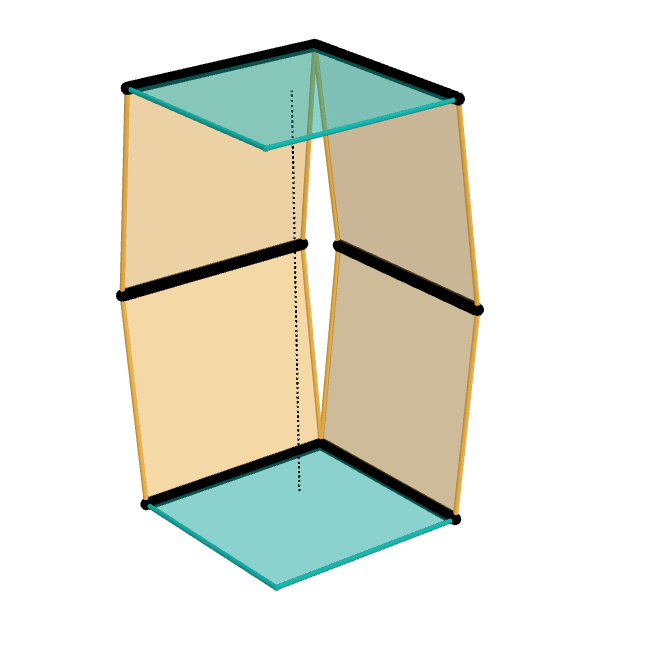
\includegraphics[width=\textwidth]{papers/geradlinig/figures/sarrus_linkage1.png}
    \end{minipage}
    \hfill
    \begin{minipage}{0.32\textwidth}
        \centering
        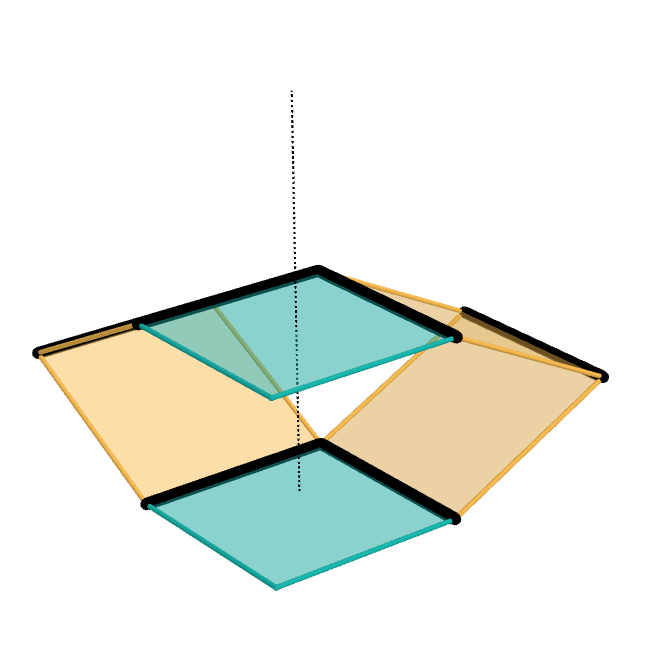
\includegraphics[width=\textwidth]{papers/geradlinig/figures/sarrus_linkage2.png}
    \end{minipage}
    \hfill
    \begin{minipage}{0.32\textwidth}
        \centering
        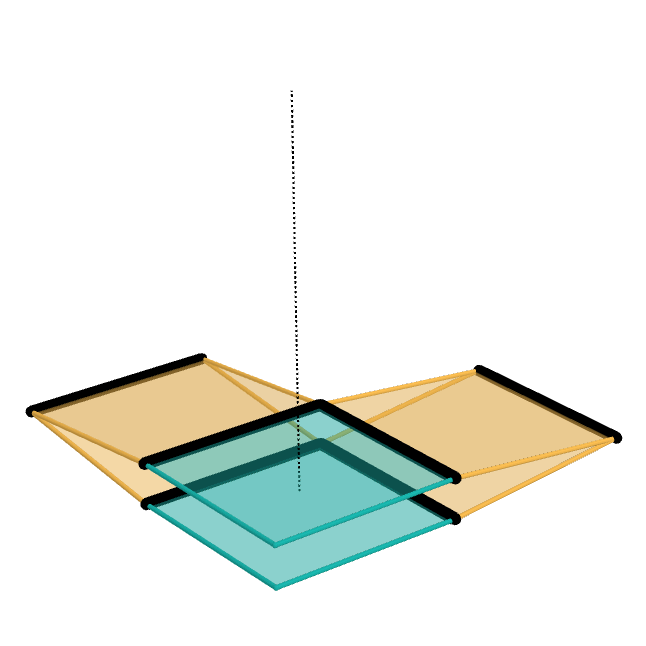
\includegraphics[width=\textwidth]{papers/geradlinig/figures/sarrus_linkage3.png}
    \end{minipage}
    \caption{Der Mechanismus von Sarrus~\cite{sarrus_linkage}.}
~\label{fig:sarrus_link}
\end{figure}

Danach erfand 1864 Charles-Nicolas Peaucellier den ersten planaren 
Mechanismus, welcher Rotationsbewegung
in eine perfekte geradlinige Bewegung umwandeln konnte,
wie in Abbildung~\ref{fig:sarrus_link} ersichtlich.
Einige Jahre nach ihm erfand Yom Tov Lipman Lipkin den
gleichen Mechanismus unabhängig von Peaucellier.
Zu ihren Ehren wird er daher der Peaucellier-Lipkin Mechanismus genannt.
\begin{figure}[htbp]
    \centering
    \begin{minipage}{0.32\textwidth}
        \centering
        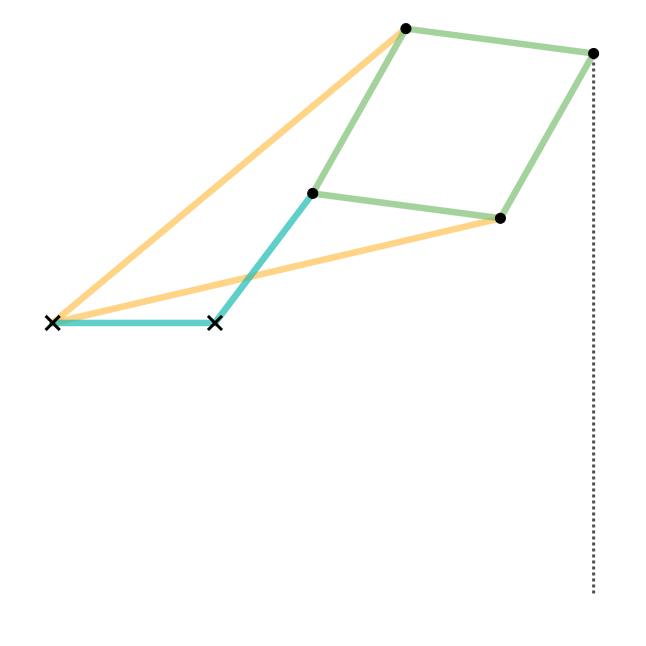
\includegraphics[width=\textwidth]{papers/geradlinig/figures/peaucellier_linkage1.png}
    \end{minipage}
    \hfill
    \begin{minipage}{0.32\textwidth}
        \centering
        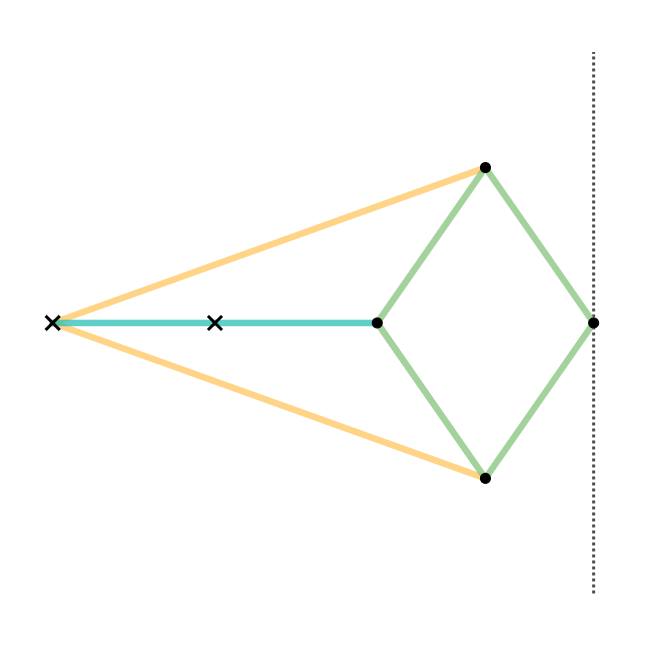
\includegraphics[width=\textwidth]{papers/geradlinig/figures/peaucellier_linkage2.png}
    \end{minipage}
    \hfill
    \begin{minipage}{0.32\textwidth}
        \centering
        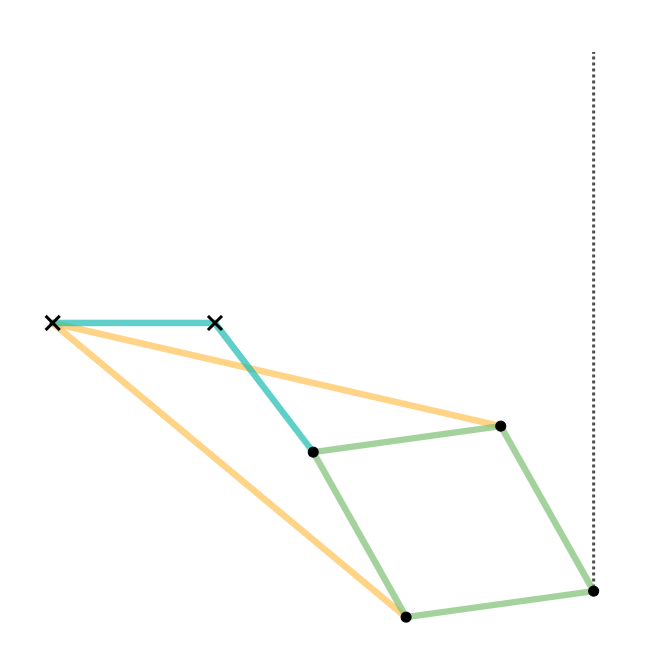
\includegraphics[width=\textwidth]{papers/geradlinig/figures/paucellier_linkage3.png}
    \end{minipage}
    \caption{Der Mechanismus von Peaucellier und Lipkin~\cite{peauc_lip_linkage}.}
~\label{fig:peaucellier_link}
\end{figure}

\subsection{Kreisspiegelung
\label{geradlinig:subsection:geometrische_inversion}}
In der geometrischen Darstellung des Peaucellier-Lipkin 
Mechanismus sind sechs Stäbe konstanter Länge 
erkennbar: $\overline{OA}$, $\overline{OC}$,
$\overline{AB}$, $\overline{BC}$, $\overline{CD}$ und $\overline{DA}$.
Die Längen von $\overline{OA}$ und $\overline{OC}$ sind gleich, und die
vier Stäbe $\overline{AB}$, $\overline{BC}$, $\overline{CD}$ und
$\overline{DA}$ besitzen ebenfalls gleiche Länge, sodass sie ein
Rhombus bilden. Der Punkt $O$ ist fest im Raum verankert.

Wird nun der Punkt $B$ dazu gezwungen, sich auf einer Kreisbahn zu
bewegen (beispielsweise durch eine zusätzliche Stange, deren Länge
halb so groß ist wie die Strecke $\overline{OB}$; die Bahn ist in Rot
dargestellt), und dieser Kreis verläuft durch den Punkt $O$, so muss
sich der Punkt $D$ notwendigerweise entlang einer Geraden bewegen
(in Blau gekennzeichnet). Im Gegensatz dazu würde sich Punkt $D$
auf einer Kreisbahn bewegen, wenn Punkt $B$ auf einer Geraden
geführt würde, die nicht durch $O$ verläuft; dieser Kreis würde
wiederum durch $O$ gehen.

Es existieren viele verschiedene Proportionen dieses Gestänges.
Da die Punkte $O$, $B$ und $D$ während der gesamten Bewegung
kollinear bleiben müssen und unzählige Kombinationen von Stablängen
möglich sind, ist eine Spiegelung des Mechanismus bezüglich der
Geraden $OBD$ nicht erforderlich. Unter der Bedingung, dass
$OBD$ stets kollinear bleibt, sind die einzigen Voraussetzungen für die
gewünschte Geradführung des Punktes $D$, dass
$\overline{AB} = \overline{AD}$ sowie $\overline{BC} = \overline{DC}$
gilt und dass Punkt $B$ auf einer Kreisbahn geführt wird, die den
Punkt $O$ schneidet. Abgesehen davon besteht keine feste Beziehung
zwischen den Längen der Seiten des Vierecks $ABCD$,
Hier die Geometrie beschreiben.
\begin{figure}[htbp]
    \centering
    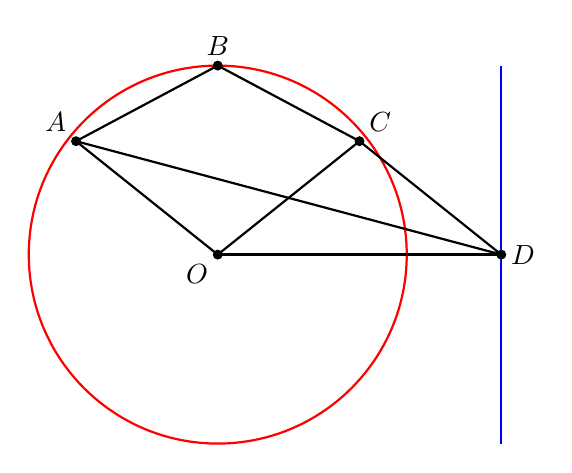
\begin{tikzpicture}[scale=1.2]
  % Circle center O and radius
  \coordinate (O) at (0,0);
  \def\r{2}

  % Circle
  \draw[red, thick] (O) circle (\r);

  % Points on/around circle (adjust as needed)
  \coordinate (A) at (-1.5,1.2);
  \coordinate (B) at (0,\r);        % top point on circle
  \coordinate (C) at (1.5,1.2);

  % Vertical line with point D to the right
  \draw[blue, thick] (3,-2) -- (3,2);
  \coordinate (D) at (3,0);

  % Quadrilateral OABC
  \draw[thick] (O) -- (A) -- (B) -- (C) -- cycle;

  % Connection to D (diamond-like shape)
  \draw[thick] (A) -- (D) -- (C);
  \draw[thick] (O) -- (D);

  % Tangent-like segments from O to A,B,C (optional emphasis)
  % (Already drawn as part of quadrilateral, but you can style them)
  % \draw[thick] (O) -- (A);
  % \draw[thick] (O) -- (B);
  % \draw[thick] (O) -- (C);

  % Mark points
  \fill (O) circle (1.5pt);
  \fill (A) circle (1.5pt);
  \fill (B) circle (1.5pt);
  \fill (C) circle (1.5pt);
  \fill (D) circle (1.5pt);

  % Labels
  \node[below left]  at (O) {$O$};
  \node[above left]  at (A) {$A$};
  \node[above]       at (B) {$B$};
  \node[above right] at (C) {$C$};
  \node[right]       at (D) {$D$};
\end{tikzpicture}

    \caption{Geometrie des Peaucellier-Lipkin Mechanismus~\cite{peauc_lip_linkage}.}
~\label{fig:perrolatz_link}
\end{figure}

Ein weiterer Mechanismus der durch Kreisspiegelung 
inspiriert wurde ist der Mechanismus von Perrolatz, 
gemäss Abbildung~\ref{fig:perrolatz_link}.

\begin{figure}[htbp]
    \centering
    \begin{minipage}{0.32\textwidth}
        \centering
        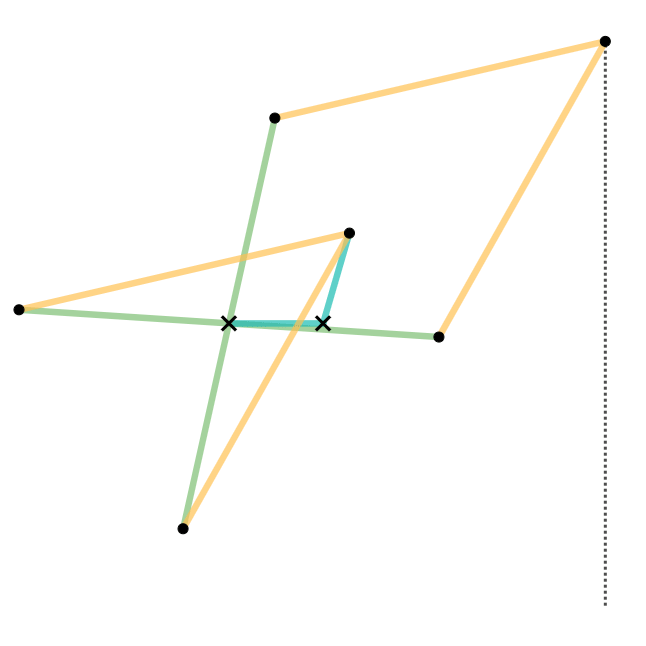
\includegraphics[width=\textwidth]{papers/geradlinig/figures/perrolatz_linkage1.png}
    \end{minipage}
    \hfill
    \begin{minipage}{0.32\textwidth}
        \centering
        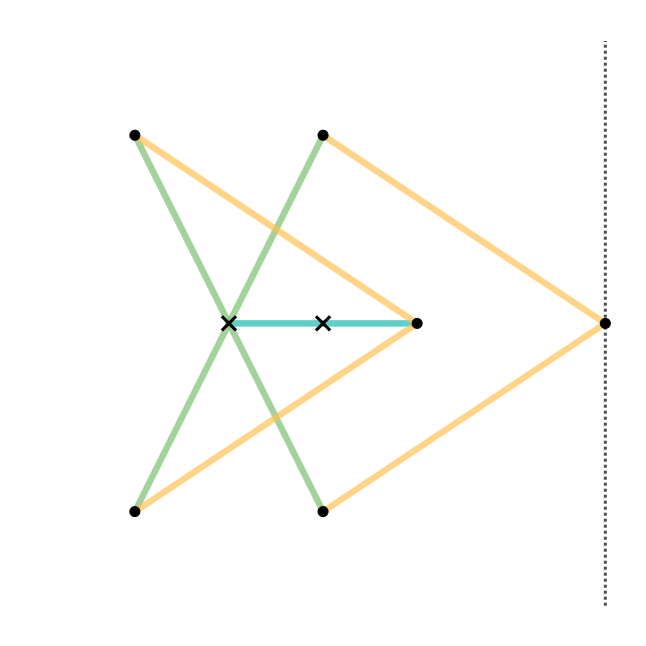
\includegraphics[width=\textwidth]{papers/geradlinig/figures/perrolatz_linkage2.png}
    \end{minipage}
    \hfill
    \begin{minipage}{0.32\textwidth}
        \centering
        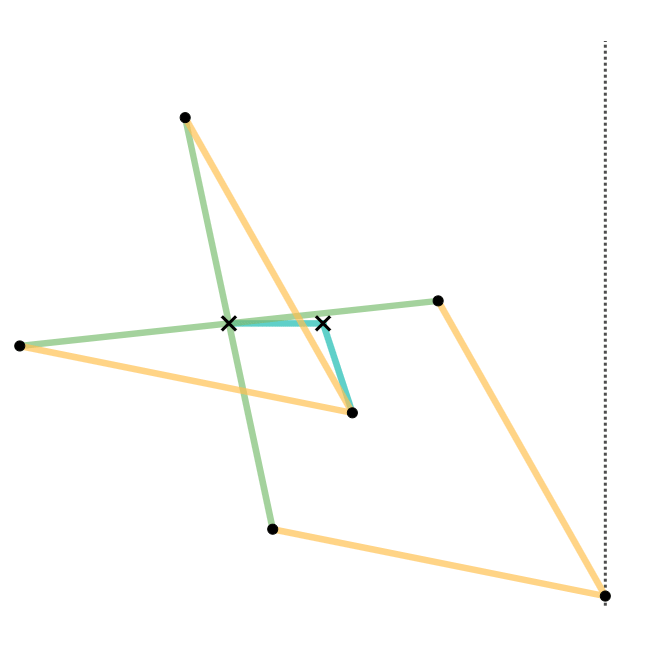
\includegraphics[width=\textwidth]{papers/geradlinig/figures/perrolatz_linkage3.png}
    \end{minipage}
    \caption{Der Mechanismus von Perrolatz~\cite{wiki_straight_line}.}
~\label{fig:perrolatz_link}
\end{figure}

